\documentclass[aspectratio=169,10pt]{beamer}

\usetheme{Madrid}
\usecolortheme{seahorse}

\usepackage[utf8]{inputenc}
\usepackage{amsmath}
\usepackage{amssymb}
\usepackage{amsfonts}
\usepackage{mathtools}
\usepackage{listings}
\usepackage{xcolor}
\usepackage{graphicx}
\usepackage{geometry}

\graphicspath{{figures/}}

% Define code style
\lstset{
  basicstyle=\ttfamily\scriptsize,
  breaklines=true,
  commentstyle=\color{green!50!black}\itshape,
  keywordstyle=\color{blue}\bfseries,
  stringstyle=\color{red},
  numbers=left,
  numberstyle=\tiny\color{gray},
  frame=single,
  language=Python,
  stepnumber=1,
  showspaces=false,
  showstringspaces=false,
  tabsize=2,
  captionpos=b
}

% Custom commands
\newcommand{\norm}[1]{\left\lVert #1 \right\rVert}
\newcommand{\abs}[1]{\left\lvert #1 \right\rvert}
\newcommand{\set}[1]{\left\{ #1 \right\}}
\newcommand{\ip}[2]{\left\langle #1, #2 \right\rangle}

% Beamer settings
\setbeamertemplate{footline}[frame number]
\setbeamerfont{block title}{size=\large, series=\bfseries}
\setbeamercolor{block title}{bg=structure.fg!20!white,fg=black}

\title{Chapter 7d: Variational Methods and Optimization}
\subtitle{Rate of Convergence and Fixed Point Theory}
\author{Based on Pathak's ``An Introduction to Nonlinear Analysis and Fixed Point Theory''}
\institute{Nonlinear Analysis and Fixed Point Theory}
\date{\today}

\begin{document}

% Title slide
\begin{frame}
  \titlepage
\end{frame}

% Outline
\begin{frame}{Outline}
  \tableofcontents
\end{frame}

% ===================================================================
% Section 1: Variational Formulation for Linear and Nonlinear Problems
% ===================================================================
\section{Variational Formulation for Linear and Nonlinear Problems}

\begin{frame}{Overview: Variational Methods}
  \begin{itemize}
    \item \textbf{Core Idea:} Transform differential equations into optimization problems
    \item \textbf{Advantage:} Direct connection between physical/mathematical problems and optimization
    \item \textbf{Framework:} Find extremal points of functionals in appropriate function spaces
    \item \textbf{Key Tools:}
    \begin{itemize}
      \item Variational calculus
      \item Functional analysis
      \item Critical point theory
    \end{itemize}
  \end{itemize}
  \vspace{0.3cm}
  \begin{block}{Definition}
    A \textbf{functional} $J: V \to \mathbb{R}$ maps functions in a Banach space $V$ to real numbers.
  \end{block}
\end{frame}

\begin{frame}{Variational Principle: From Calculus of Variations}
  \begin{columns}
    \column{0.5\textwidth}
    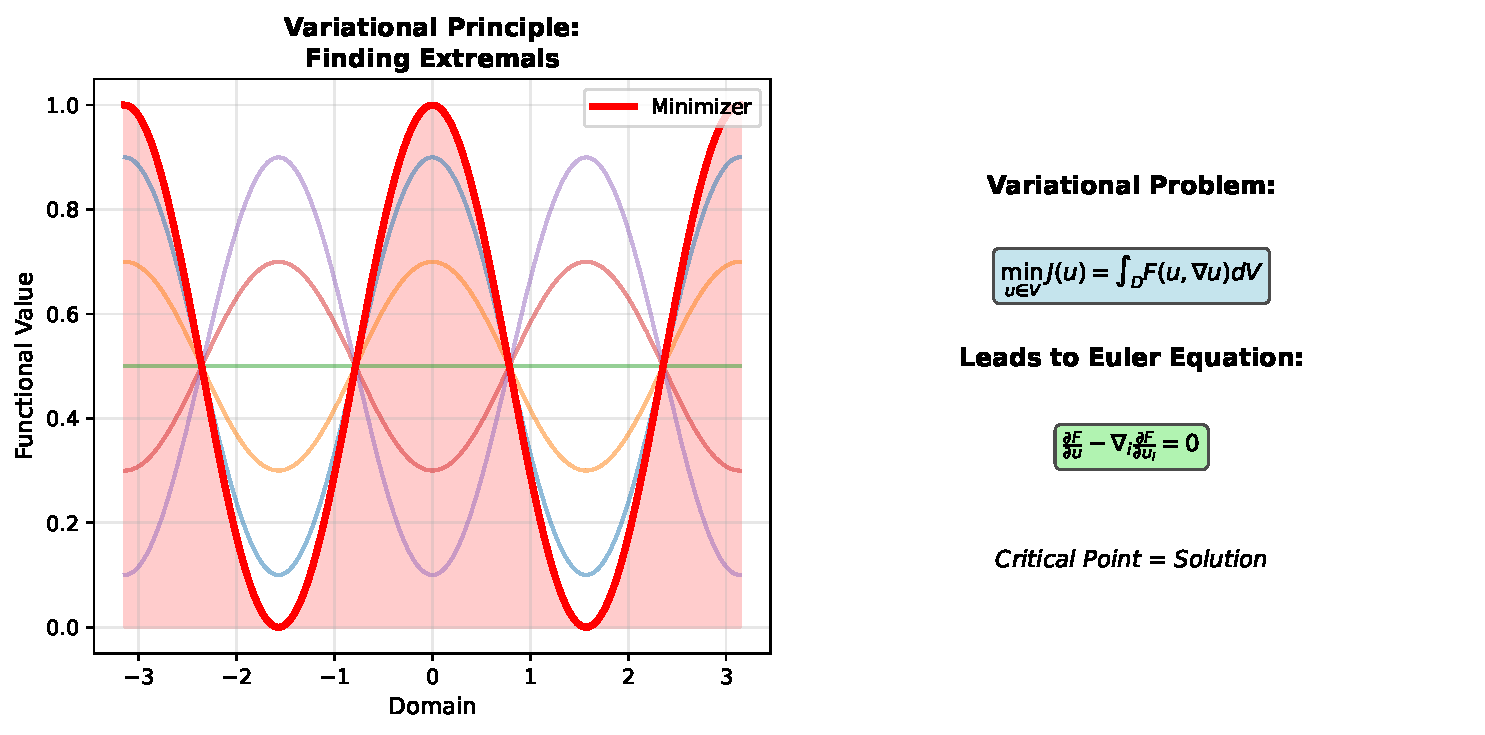
\includegraphics[width=\textwidth]{variational_principle.pdf}

    \column{0.5\textwidth}
    \textbf{Classical Problem:} Find the minimum of
    \[
      J(u) = \int_D F(u, \nabla u) \, dV
    \]
    subject to boundary conditions on $\partial D$.

    \vspace{0.3cm}
    \textbf{Solution Method:}
    \begin{enumerate}
      \item Compute the first variation: $\delta J = 0$
      \item Derive Euler-Lagrange equation
      \item Solve for critical points
    \end{enumerate}
  \end{columns}
\end{frame}

\begin{frame}[fragile]{Variational Problems: Concrete Example}
  \textbf{Problem:} Find extremals of the functional
  \[
    I[y(x)] = \int x\sqrt{1 + y'^2} \, dx
  \]

  \vspace{0.3cm}
  \textbf{Solution Steps:}
  \begin{enumerate}
    \item Here $F(x, y, y') = x\sqrt{1 + y'^2}$
    \item Euler equation: $F_y - \frac{d}{dx}F_{y'} = 0$
    \item Compute: $F_y = 0$, \quad $F_{y'} = \frac{xy'}{\sqrt{1 + y'^2}}$
    \item This gives: $\frac{d}{dx}\left(\frac{xy'}{\sqrt{1 + y'^2}}\right) = 0$
  \end{enumerate}

  \vspace{0.3cm}
  \textbf{Result:} The extremals are parabolas: $(y - c_1)^2 = 4c_2(x - c_2)$
\end{frame}

\begin{frame}{Symmetry and Self-Adjoint Operators}
  \textbf{Key Observation:} A variational principle exists if and only if the operator is self-adjoint.

  \vspace{0.3cm}
  For an operator $P: X \to X^*$ (where $X^*$ is the dual space), the \textbf{symmetry condition} is:
  \[
    \int \Psi P'_u \phi \, dV = \int \phi P'_u \Psi \, dV
  \]

  \vspace{0.3cm}
  \begin{block}{Theorem 7.18 (Vainberg)}
    Suppose:
    \begin{enumerate}
      \item $P: X \to X^*$ is an operator from normed space $X$ to its conjugate
      \item $P$ has a linear Gâteaux differential at every point
      \item The bilinear functional $(DP(x, h_1), h_2)$ is continuous in $x$
    \end{enumerate}
    Then $P$ is potential (i.e., $P = \nabla F$) iff the symmetry condition holds.
  \end{block}
\end{frame}

\begin{frame}{Functional Formulation of Differential Equations}
  \textbf{Problem:} Given a differential equation $P(u) = f$ in domain $D$

  \textbf{Variational Reformulation:}
  \[
    \min_{u \in V} J(u) = \int_D \left[P(u) - f\right]^2 dV
  \]

  \vspace{0.2cm}
  \textbf{Example:} For Poisson equation $-\Delta u = f$:
  \[
    J(u) = \int_D \left[\norm{\nabla u}^2 - 2fu\right] dV \quad \text{(Dirichlet form)}
  \]

  \vspace{0.3cm}
  \begin{block}{Least Squares Method}
    For non-self-adjoint operators, the least squares variational formulation is:
    \[
      J(u) = \int_D (Lu - f)^2 \, dV
    \]
    which minimizes the $L^2$ residual.
  \end{block}
\end{frame}

\begin{frame}{Gâteaux and Fréchet Derivatives}
  \textbf{Gâteaux Derivative:} For a functional $F: X \to \mathbb{R}$:
  \[
    F'_u(h) = \lim_{\varepsilon \to 0} \frac{F(u + \varepsilon h) - F(u)}{\varepsilon}
  \]
  directional derivative in direction $h$

  \vspace{0.3cm}
  \textbf{Fréchet Derivative:} A continuous linear operator $A \in \mathcal{L}(X, Y)$ such that:
  \[
    \lim_{h \to 0} \frac{\norm{F(x + h) - F(x) - Ah}}{\norm{h}} = 0
  \]

  \vspace{0.3cm}
  \begin{itemize}
    \item \textbf{Fréchet} $\Rightarrow$ \textbf{Gâteaux} (always)
    \item \textbf{Gâteaux} $\Rightarrow$ \textbf{Fréchet} (under continuity conditions)
  \end{itemize}
\end{frame}

% ===================================================================
% Section 2: Mountain Pass Lemma and Critical Points
% ===================================================================
\section{Mountain Pass Lemma and Critical Points}

\begin{frame}{Mountain Pass Lemma (MPL)}
  \begin{columns}
    \begin{column}{0.5\textwidth}
      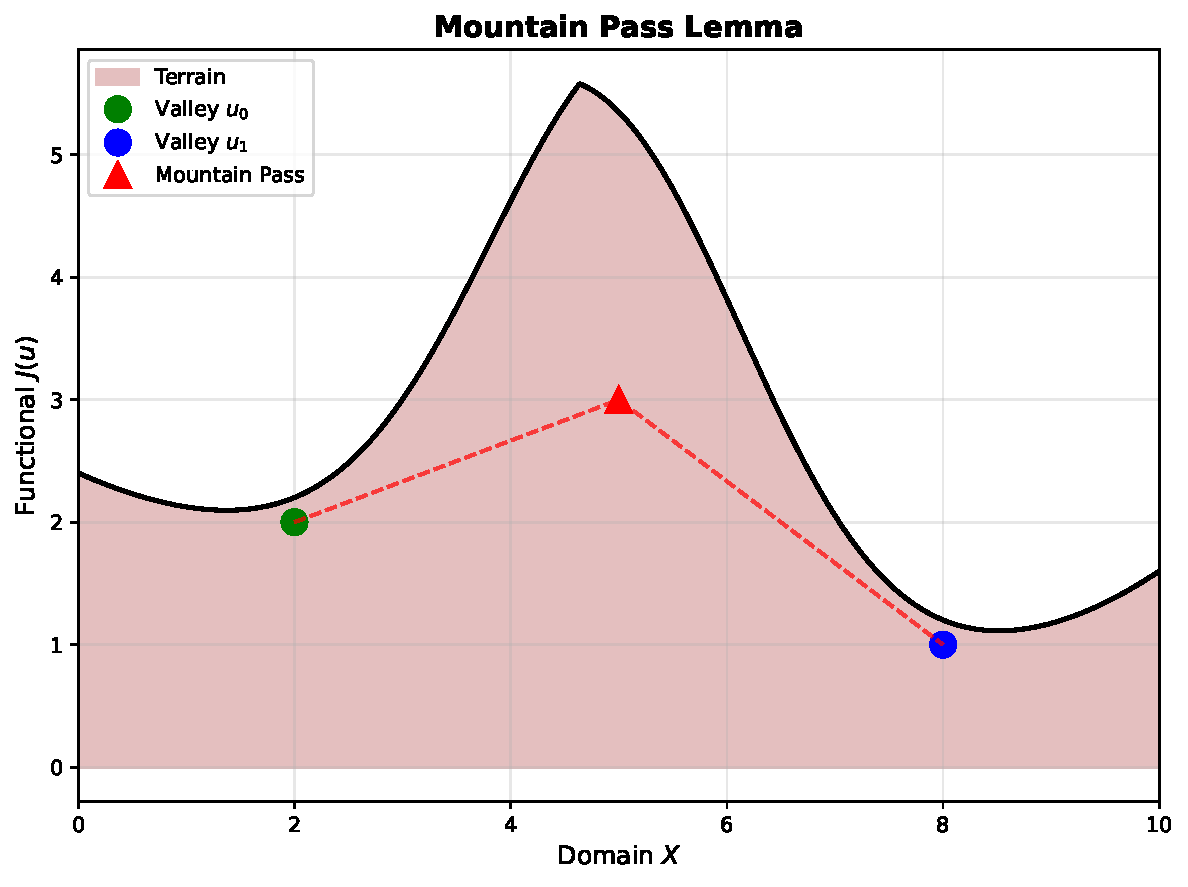
\includegraphics[width=\textwidth]{mountain_pass.pdf}
    \end{column}

    \begin{column}{0.5\textwidth}
      \textbf{Intuition:} To go from one valley to another, we must cross a mountain pass.

      \vspace{0.3cm}
      \textbf{Formal Statement:}
      Let $J: X \to \mathbb{R}$ be a $C^1$ functional. Suppose:
      \begin{enumerate}
        \item $\norm{u_1 - u_0} > R_1$
        \item $J(u_0), J(u_1) < c_0 \leq \inf_{\norm{v - u_0} = R_1} J(v)$
      \end{enumerate}
      Then $J$ has a critical value $c \geq c_0$ defined by:
      \[
        c = \inf_p \max_{u \in p} J(u)
      \]
    \end{column}
  \end{columns}
\end{frame}

\begin{frame}{Palais-Smale Condition}
  \textbf{Problem with MPL:} The conclusion doesn't always hold!

  \vspace{0.2cm}
  \textbf{Counterexample:} $F(z) = |e^z - 1|^4$ on $\mathbb{C}$
  \begin{itemize}
    \item Minima at $z = 0$ and $2\pi i$
    \item Only critical value is at 0
    \item The mountain at $\pi i$ exists but is not critical
  \end{itemize}

  \vspace{0.3cm}
  \begin{block}{Palais-Smale (PS) Condition}
    Any sequence $\{u_i\}$ in $X$ for which:
    \begin{enumerate}
      \item $J(u_i) \to c$ (bounded)
      \item $J'(u_i) \to 0$ (derivatives vanish)
    \end{enumerate}
    has a strongly convergent subsequence.
  \end{block}

  \textbf{Conclusion:} With PS condition, MPL guarantees a critical point at the mountain pass!
\end{frame}

\begin{frame}{Example: Finding Critical Points}
  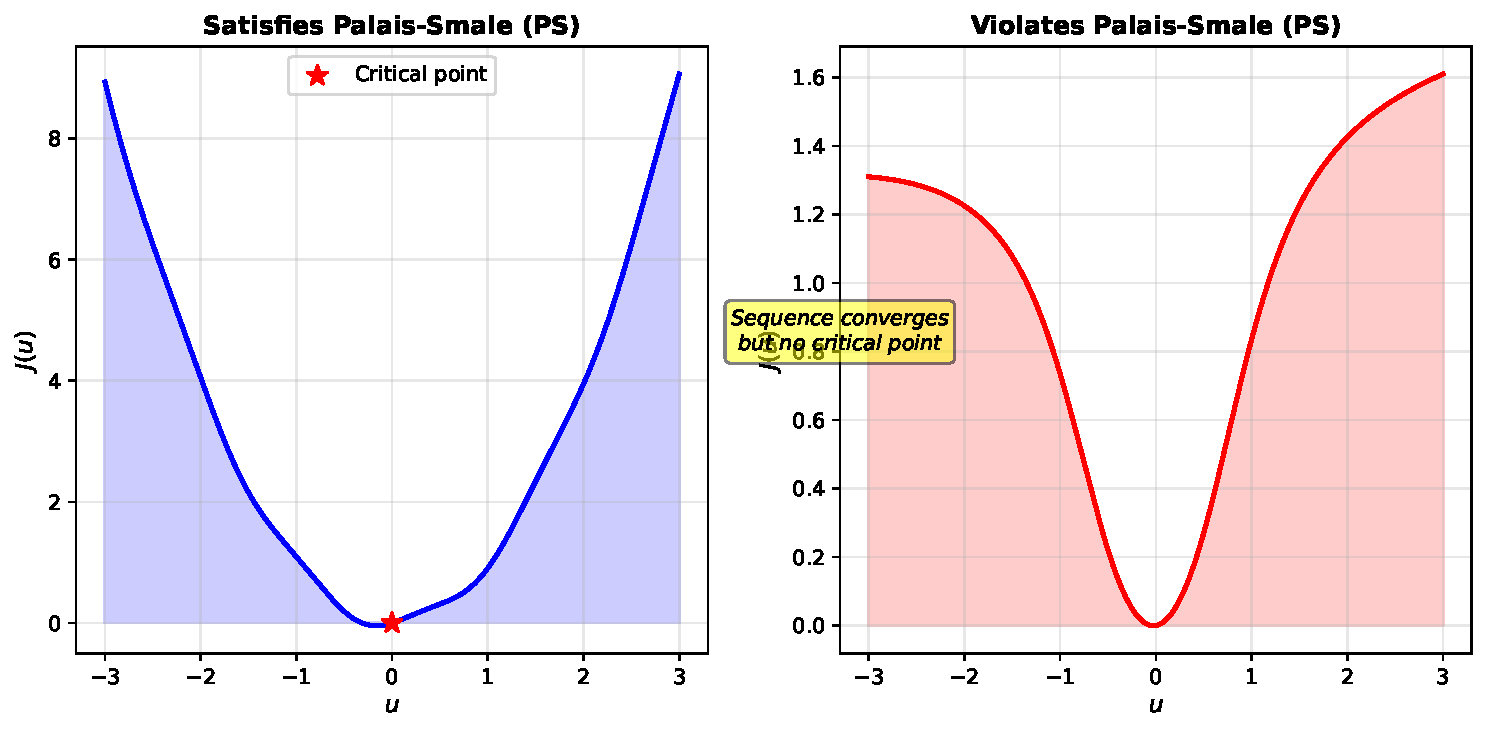
\includegraphics[width=\textwidth]{palais_smale.pdf}
\end{frame}

% ===================================================================
% Section 3: Variational Principles for Non-self-adjoint Equations
% ===================================================================
\section{Variational Principles for Non-self-adjoint Equations}

\begin{frame}{Adjoint Operators}
  \textbf{Definition:} For operator $A: \mathcal{H} \to \mathcal{H}$, the \textbf{adjoint} $A^*$ satisfies:
  \[
    (Ax, y) = (x, A^*y) \quad \forall x, y \in \mathcal{H}
  \]

  \vspace{0.3cm}
  \textbf{Self-Adjoint:} $A = A^*$

  \vspace{0.3cm}
  \textbf{Problem:} Non-self-adjoint equations don't admit variational principles directly!

  \vspace{0.3cm}
  \textbf{Solution:} Transform via least squares:
  \[
    J(u) = \int_V (Lu - f)^2 dV
  \]
  This is always variational, even for non-self-adjoint $L$.

  \vspace{0.3cm}
  \begin{block}{Key Insight}
    The minimum of $J(u) = \int_V (Lu - f)^2 dV$ gives a least-squares solution, even when $L$ is not self-adjoint.
  \end{block}
\end{frame}

\begin{frame}{Boundary Value Problems}
  \textbf{General Boundary Value Problem:}
  \begin{align}
    Lu = f & \quad \text{in } V \label{eq:bvp1} \\
    B_i u = 0 & \quad \text{on } S \label{eq:bvp2}
  \end{align}

  where $S$ is the piecewise smooth boundary of domain $V$.

  \vspace{0.3cm}
  \textbf{When $L$ is self-adjoint:}
  \[
    J(u) = \frac{1}{2}\int_V uLu \, dV \quad \Rightarrow \quad \min J \text{ gives solution}
  \]

  \vspace{0.3cm}
  \textbf{When $L$ is non-self-adjoint:}
  \[
    J(u) = \int_V (Lu - f)^2 dV \quad \Rightarrow \quad \min J \text{ gives least-squares solution}
  \]
\end{frame}

% ===================================================================
% Section 4: Hamiltonian Systems and Hamilton's Equations
% ===================================================================
\section{Hamiltonian Systems and Canonical Equations}

\begin{frame}{Hamiltonian Formulation}
  \textbf{Classical Problem:} Second-order equation $T^* T q = f$

  \vspace{0.3cm}
  \textbf{Hamiltonian Reformulation:} Split into first-order system:
  \begin{align}
    Tx &= \rho \\
    T^* \rho &= f
  \end{align}

  where $\rho$ represents generalized momentum.

  \vspace{0.3cm}
  \textbf{Hilbert Space Formulation:} Let $\mathcal{H} = \mathcal{H}_1 \oplus \mathcal{H}_2$, then:
  \[
    L(x, Tx) = (Tx, \tilde{p}) - \frac{1}{2}(\tilde{p}, \tilde{p}) - (f, x)
  \]

  \vspace{0.3cm}
  \begin{block}{Hamilton's Canonical Equations}
    \[
      Tx = W_p, \quad T^*p = W_x
    \]
    where $W(x, p) = \frac{1}{2}(p, p) + (f, x)$
  \end{block}
\end{frame}

\begin{frame}{Hamiltonian Phase Space Dynamics}
  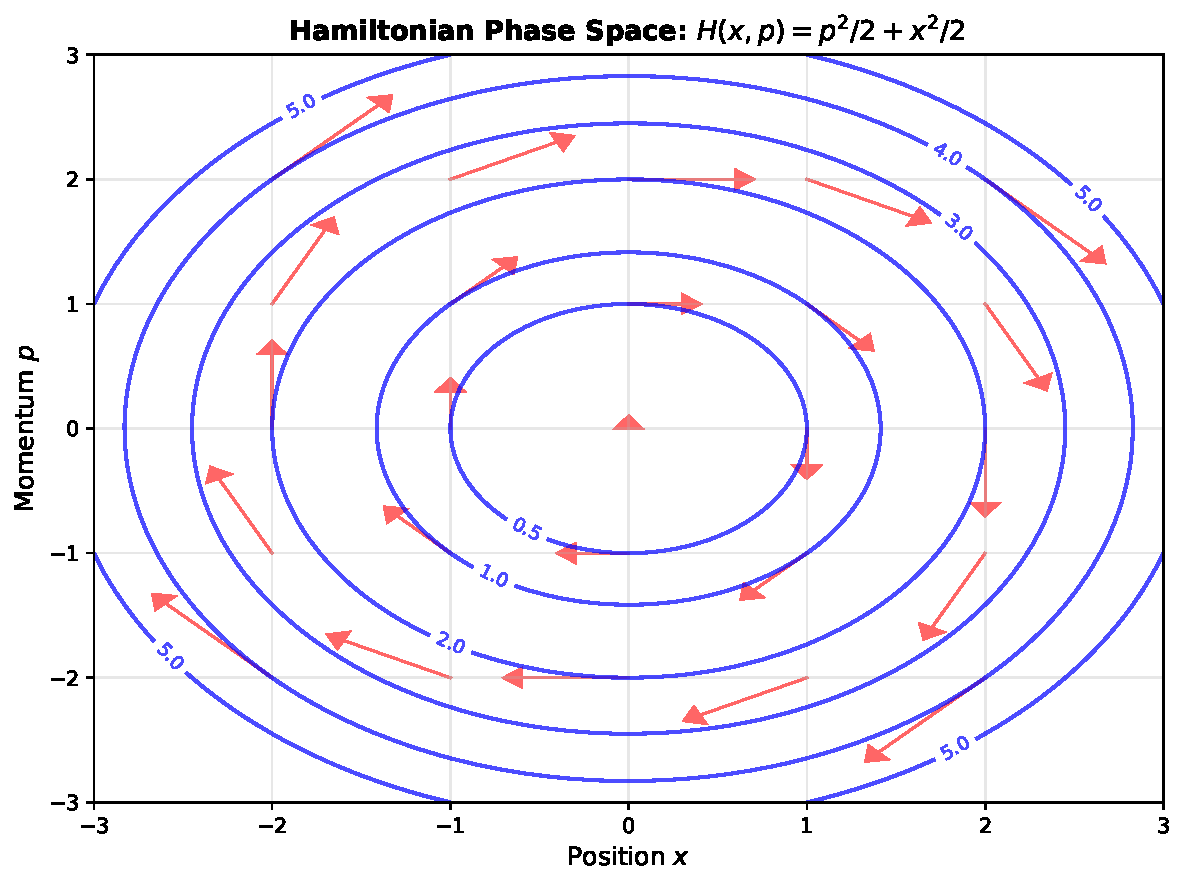
\includegraphics[width=\textwidth]{hamiltonian_phase_space.pdf}

  \vspace{0.2cm}
  \textbf{Key Features:}
  \begin{itemize}
    \item Level sets of Hamiltonian are invariant (conserved quantities)
    \item Trajectories follow contours of constant energy
    \item Symplectic structure preserves phase space volume
  \end{itemize}
\end{frame}

\begin{frame}{Lagrangian and Hamiltonian Duality}
  \textbf{Legendre Transformation:} The duality between Lagrangian and Hamiltonian:
  \[
    \mathcal{H} = L - (Aq, p)
  \]

  where $p = \frac{\partial L}{\partial(Aq)}$

  \vspace{0.3cm}
  \textbf{Connection:}
  \begin{itemize}
    \item Lagrangian: $\min J = \int L(q, \dot{q}) \, dt$
    \item Hamiltonian: Reformulate using conjugate momentum $p$
    \item Both describe same dynamics: $Tq = p(t)$, $T^*p = f(q(t),t)$
  \end{itemize}

  \vspace{0.3cm}
  \begin{block}{Mechanics Analogy}
    \begin{itemize}
      \item $x$ = generalized displacement
      \item $p = T^*x'$ = generalized momentum
      \item $\mathcal{H} = \frac{1}{2}(p,p) + V(x)$ = total energy
    \end{itemize}
  \end{block}
\end{frame}

% ===================================================================
% Section 5: Applications to Quantum Mechanics
% ===================================================================
\section{Quantum Mechanics via Variational Principles}

\begin{frame}{Schrödinger Equation from Variational Principle}
  \textbf{Problem:} Find wave function $\Psi$ that extremizes:
  \[
    \int_D \Psi^*(\mathcal{H}\Psi) \, dxdydz
  \]
  subject to normalization $\int_D \Psi^*\Psi \, dxdydz = 1$

  \vspace{0.3cm}
  where $\mathcal{H} = -k\nabla^2 + V(x,y,z)$ is the Hamiltonian operator.

  \vspace{0.3cm}
  \textbf{Solution Method:}
  \begin{enumerate}
    \item Introduce Lagrange multiplier $\lambda$ for constraint
    \item Compute Euler equations
    \item Result: $-k\nabla^2\Psi + V\Psi = \lambda\Psi$
  \end{enumerate}

  \vspace{0.3cm}
  \textbf{Conclusion:} The time-independent Schrödinger equation is an eigenvalue problem!
\end{frame}

\begin{frame}{Schrödinger Equation Example}
  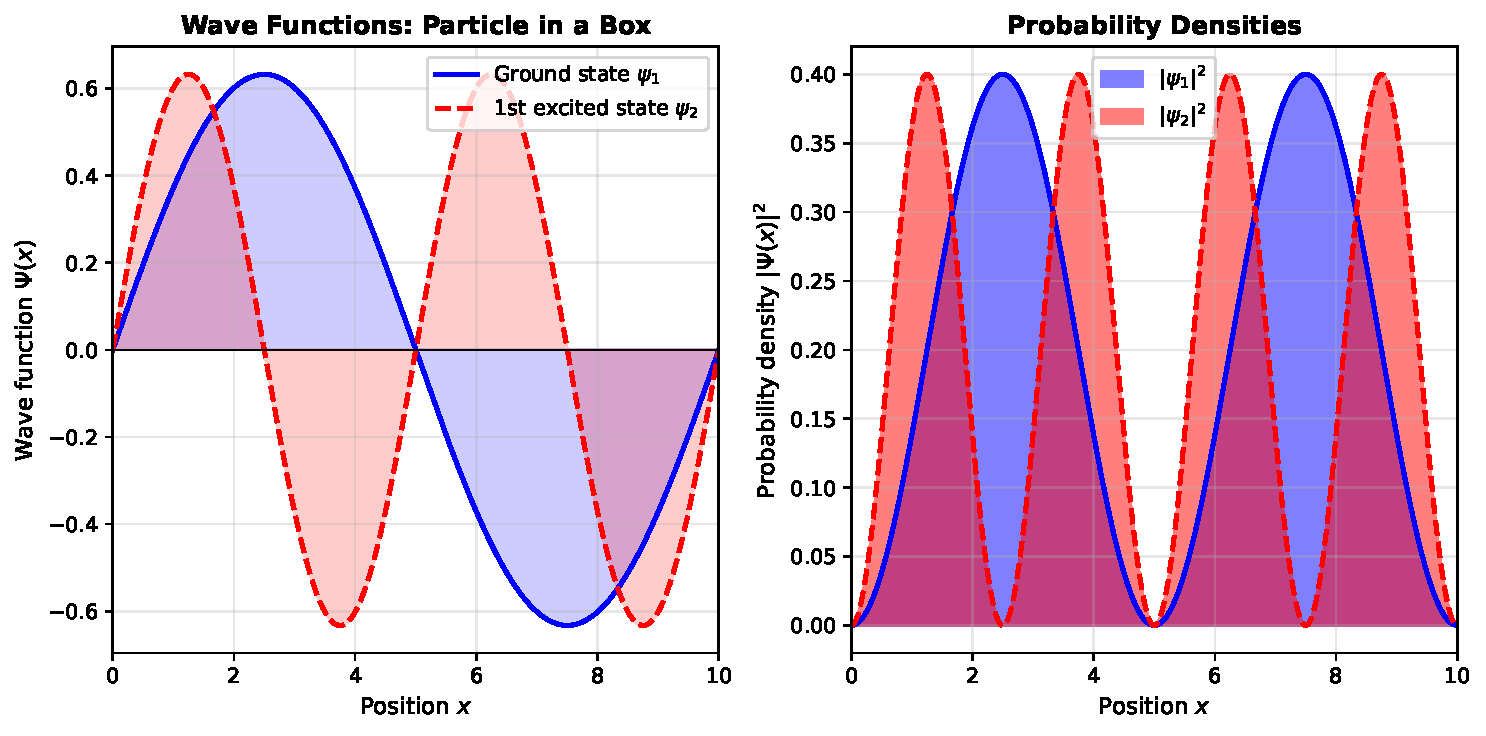
\includegraphics[width=\textwidth]{schrodinger_solutions.pdf}

  \vspace{0.2cm}
  \textbf{Particle in a Box:} Ground and first excited states showing wave-particle duality
\end{frame}

\begin{frame}{Klein-Gordon Equation}
  \textbf{Relativistic Wave Equation:}
  \[
    \nabla^2\Psi - \frac{1}{c^2}\frac{\partial^2\Psi}{\partial t^2} - \left(\frac{mc}{\hbar}\right)^2\Psi = 0
  \]

  \vspace{0.3cm}
  \textbf{Variational Formulation:} Lagrangian density:
  \[
    L = -\frac{\hbar^2}{2m}\left[\nabla\Psi^* \cdot \nabla\Psi - \frac{1}{c^2}\left(\frac{\partial\Psi}{\partial t}\right)^2 + \left(\frac{mc}{\hbar}\right)^2\Psi^*\Psi\right]
  \]

  \vspace{0.3cm}
  \begin{itemize}
    \item Minimizing action $\int L \, dtdx$ yields Klein-Gordon equation
    \item Extends Schrödinger to relativistic domain
    \item Predicts antiparticles (hole theory)
  \end{itemize}
\end{frame}

% ===================================================================
% Section 6: Convergence of Fixed Points
% ===================================================================
\section{Rate of Convergence for Fixed Point Iterations}

\begin{frame}{Fixed Point Problems}
  \textbf{Abstract Fixed Point Problem:} Find $x^* \in X$ such that:
  \[
    x^* = T(x^*)
  \]

  where $T: X \to X$ is a mapping on Banach space $X$.

  \vspace{0.3cm}
  \textbf{Iterative Solution:}
  \[
    x_{n+1} = T(x_n)
  \]

  \vspace{0.3cm}
  \begin{block}{Fundamental Questions}
    \begin{enumerate}
      \item Does $\{x_n\}$ converge to $x^*$?
      \item How fast does it converge?
      \item Can we characterize the convergence rate?
    \end{enumerate}
  \end{block}
\end{frame}

\begin{frame}{Convergence Rates}
  
\includegraphics[width=\textwidth]{convergence_rates.pdf}
\end{frame}

\begin{frame}{Convergence Rate Definitions}
  \textbf{Error:} $e_n = \norm{x_n - x^*}$

  \vspace{0.3cm}
  \textbf{Linear Convergence:}
  \[
    \limsup_{n \to \infty} \frac{e_{n+1}}{e_n} = r < 1
  \]
  \begin{itemize}
    \item $e_n \sim C \cdot r^n$ for some constant $C$
    \item Slowest rate (exponential decay)
  \end{itemize}

  \vspace{0.3cm}
  \textbf{Superlinear Convergence:}
  \[
    \lim_{n \to \infty} \frac{e_{n+1}}{e_n} = 0
  \]

  \vspace{0.3cm}
  \textbf{Quadratic Convergence:}
  \[
    \limsup_{n \to \infty} \frac{e_{n+1}}{e_n^2} = C < \infty
  \]
  \begin{itemize}
    \item Exponential improvement: errors square at each step
    \item Fastest practical rate
  \end{itemize}
\end{frame}

\begin{frame}{Contraction Mapping Theorem and Convergence}
  \begin{block}{Banach Contraction Mapping Theorem}
    If $T: X \to X$ is a contraction mapping with constant $L < 1$:
    \[
      \norm{T(x) - T(y)} \leq L\norm{x - y} \quad \forall x,y \in X
    \]
    Then there exists unique fixed point $x^* = T(x^*)$ and:
    \[
      \norm{x_n - x^*} \leq \frac{L^n}{1-L}\norm{x_1 - x_0}
    \]
  \end{block}

  \vspace{0.3cm}
  \textbf{Conclusion:} Contraction mappings guarantee \textbf{linear convergence} with rate $r = L$.

  \vspace{0.3cm}
  \textbf{Faster Rates:} For non-contractive mappings (like Newton's method):
  \begin{itemize}
    \item Requires stronger conditions (e.g., differentiability)
    \item Can achieve quadratic or superlinear convergence
  \end{itemize}
\end{frame}

\begin{frame}{Functional Evolution During Convergence}
  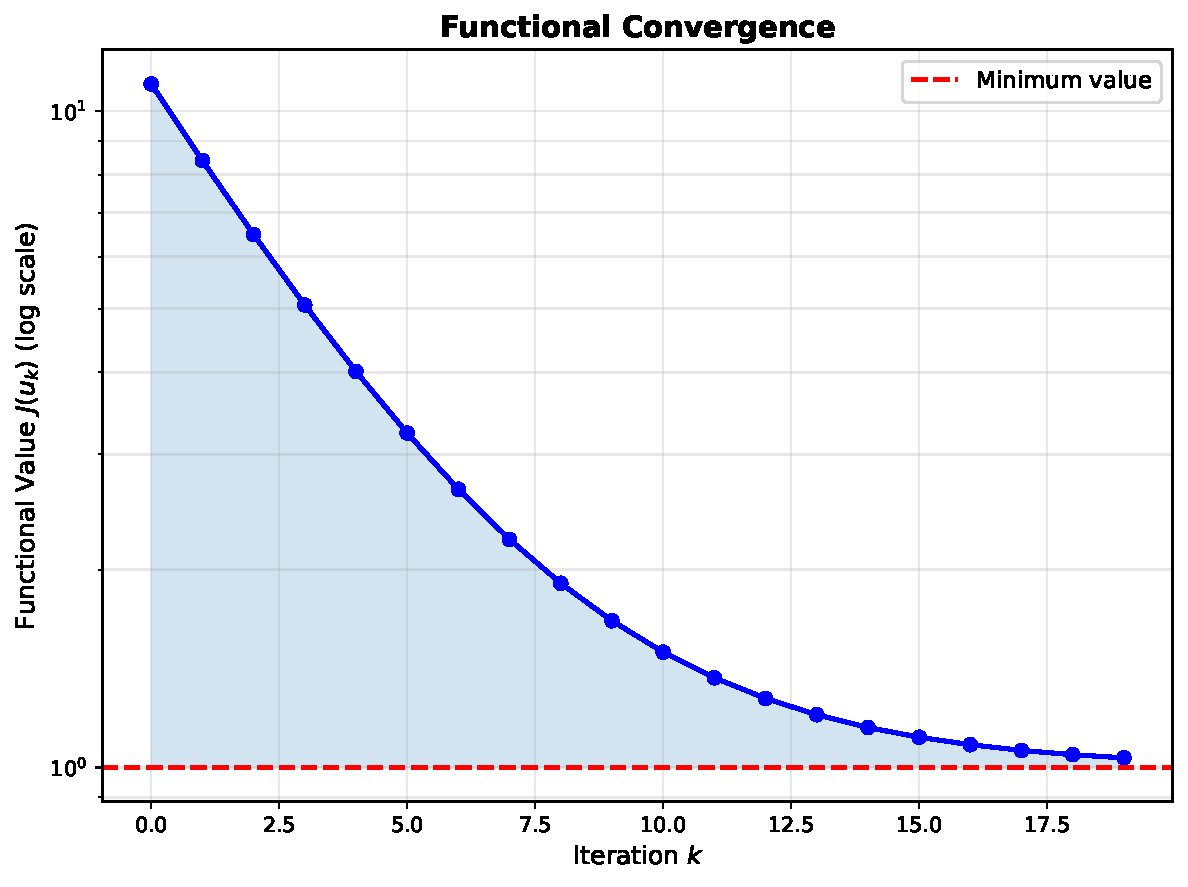
\includegraphics[width=\textwidth]{functional_evolution.pdf}

  \vspace{0.2cm}
  \textbf{Observation:} The functional $J(u_k)$ monotonically decreases and converges to minimum value
\end{frame}

% ===================================================================
% Section 7: Numerical Examples and Applications
% ===================================================================
\section{Numerical Examples}

\begin{frame}[fragile]{Example: Euler-Lagrange Equation}
  \textbf{Problem:} Find extremals of the functional
  \[
    I[y(x)] = \int_0^1 (y'^2 + y^2 + 1) \, dx, \quad y(0)=1, \quad y(1)=2
  \]

  \vspace{0.2cm}
  \textbf{Solution Process:}
  \begin{enumerate}
    \item Identify: $F(x,y,y') = y'^2 + y^2 + 1$
    \item Compute: $F_y = 2y$, \quad $F_{y'} = 2y'$
    \item Euler equation: $2y - \frac{d}{dx}(2y') = 0 \Rightarrow y'' - y = 0$
    \item General solution: $y = c_1 e^x + c_2 e^{-x}$
    \item Apply BC: $c_1 + c_2 = 1$, $c_1 e + c_2 e^{-1} = 2$
  \end{enumerate}

  \vspace{0.3cm}
  \textbf{Result:} Explicit formula for extremal on interval $[0,1]$
\end{frame}

\begin{frame}{Example: Minimum Surface Area (Catenary)}
  \textbf{Problem:} Curve of revolution with minimum surface area connecting two circles.

  \vspace{0.3cm}
  \textbf{Surface Area Functional:}
  \[
    A = \int_{x_1}^{x_2} 2\pi x\sqrt{1 + y'^2(x)} \, dx
  \]

  \vspace{0.3cm}
  \textbf{Euler Equation:} For $F = x\sqrt{1 + y'^2}$:
  \[
    \frac{d}{dx}\left(\frac{xy'}{\sqrt{1 + y'^2}}\right) = \sqrt{1 + y'^2}
  \]

  \vspace{0.3cm}
  \textbf{Solution:} The catenary curve
  \[
    y(x) = c_1 \cosh^{-1}\left(\frac{x}{c_1}\right) + c_2
  \]

  \textbf{Physical Application:} Shape of hanging cable under gravity!
\end{frame}

\begin{frame}[fragile]{Rayleigh-Ritz Method for Eigenvalues}
  \textbf{Problem:} Approximate the first eigenvalue of $\nabla^2 z + \lambda z = 0$ in circle of radius 1.

  \vspace{0.3cm}
  \textbf{Rayleigh-Ritz Approach:}
  \begin{enumerate}
    \item Choose ansatz: $z(x,y) = (1 - r^2)$
    \item Compute Rayleigh quotient: $\lambda \approx \frac{\int_D (\nabla z)^2 dA}{\int_D z^2 dA}$
    \item Result: $\lambda_1 \approx 10.02$ (exact: $\approx 10.17$)
  \end{enumerate}

  \vspace{0.3cm}
  \textbf{Algorithm Structure:}
  \begin{lstlisting}
def rayleigh_ritz(domain, ansatz_basis, bvp_params):
    # Compute stiffness matrix K
    K = assemble(grad(phi) * grad(phi))

    # Compute mass matrix M
    M = assemble(phi * phi)

    # Solve generalized eigenvalue problem
    eigvals, eigvecs = eig(K, M)

    return min(eigvals)  # Approximation
  \end{lstlisting}
\end{frame}

% ===================================================================
% Section 8: Summary and Advanced Topics
% ===================================================================
\section{Summary and Perspectives}

\begin{frame}{Key Takeaways}
  \begin{enumerate}
    \item \textbf{Variational Framework:} Differential equations $\leftrightarrow$ Minimization problems

    \item \textbf{Functional Analysis:} Extension of calculus to infinite-dimensional spaces

    \item \textbf{Mountain Pass Lemma:} Geometric principle for finding critical points (solutions)

    \item \textbf{Hamiltonian Systems:} Unifies classical mechanics and quantum mechanics

    \item \textbf{Convergence Theory:} Quantifies how fast iterative methods reach fixed points

    \item \textbf{Applications:} Physics, mechanics, quantum mechanics, optimization
  \end{enumerate}
\end{frame}

\begin{frame}{Connection to Fixed Point Theory}
  \textbf{Fixed Point Iteration:}
  \[
    x_{n+1} = T(x_n) \quad \Rightarrow \quad x_n \to x^* \text{ where } T(x^*) = x^*
  \]

  \vspace{0.3cm}
  \textbf{Variational Perspective:} Can reformulate as:
  \[
    \min_{x} \norm{x - T(x)}^2
  \]

  \vspace{0.3cm}
  \textbf{Convergence Rate Analysis:}
  \begin{itemize}
    \item \textbf{Contraction:} Rate depends on contraction constant
    \item \textbf{Non-smooth:} Can use variational methods to analyze rate
    \item \textbf{Quasi-linear:} Intermediate cases between linear and quadratic
  \end{itemize}

  \vspace{0.3cm}
  \textbf{Advanced Topic:} Modern variational methods use first-order optimization:
  \begin{itemize}
    \item Gradient descent
    \item Proximal algorithms
    \item Splitting methods (ADMM, etc.)
  \end{itemize}
\end{frame}

\begin{frame}{Further Reading and Resources}
  \begin{itemize}
    \item \textbf{Pathak (2018):} ``An Introduction to Nonlinear Analysis and Fixed Point Theory''

    \item \textbf{Variational Methods:}
    \begin{itemize}
      \item Evans, L. C. (1998): ``Partial Differential Equations''
      \item Dacorogna, B. (2008): ``Direct Methods in the Calculus of Variations''
    \end{itemize}

    \item \textbf{Functional Analysis:}
    \begin{itemize}
      \item Rudin, W. (1991): ``Functional Analysis''
      \item Brezis, H. (2011): ``Functional Analysis, Sobolev Spaces and PDEs''
    \end{itemize}

    \item \textbf{Computational Methods:}
    \begin{itemize}
      \item Nocedal \& Wright (2006): ``Numerical Optimization''
      \item Boyd \& Parikh (2011): ``Proximal Algorithms''
    \end{itemize}
  \end{itemize}
\end{frame}

\begin{frame}[fragile]{Code: Simple Fixed Point Iteration}
  \begin{lstlisting}
import numpy as np

def fixed_point_iteration(T, x0, tol=1e-10,
                          maxiter=1000):
    x = x0
    errors = [np.linalg.norm(x - T(x))]

    for k in range(maxiter):
        x_new = T(x)
        error = np.linalg.norm(x_new - x)
        errors.append(error)
        if error < tol:
            return x_new, errors
        x = x_new
    return x, errors

# Newton's method for sqrt(2)
def sqrt_iter(x, a=2):
    return 0.5 * (x + a / x)

x_final, errs = fixed_point_iteration(
    lambda x: sqrt_iter(x, 2.0), x0=1.0)
print(f"sqrt(2) = {x_final:.15f}")
  \end{lstlisting}
\end{frame}

\end{document}
